\begingroup
\setmainfont{DejaVu Sans}

\resizebox{\linewidth}{!}{
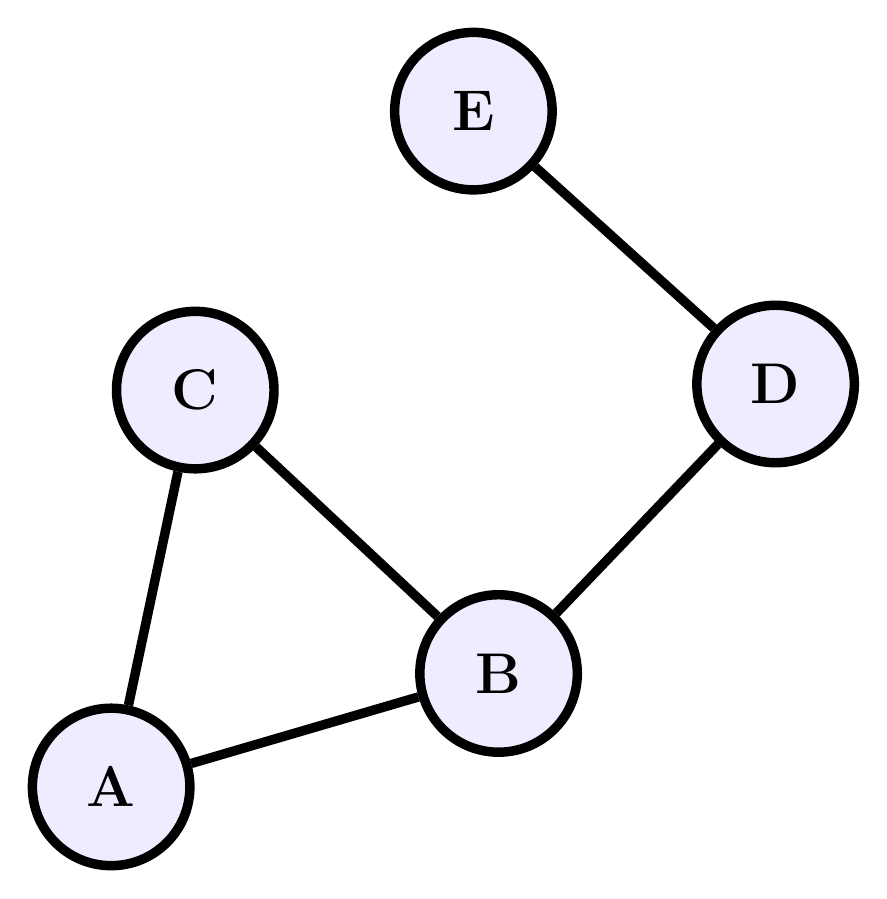
\begin{tikzpicture}

  \tikzset{
    mynode/.style={
      circle,
      draw=black,
      fill=blue!7,
      line width=1.2mm,
      minimum size=20mm,
      font=\bfseries\fontsize{20}{20}\selectfont,
      text centered
    }
  }

  \node[mynode] (A) at (110.1pt, 106.1pt) {A};
  \node[mynode] (B) at (250.1pt, 147.1pt) {B};
  \node[mynode] (C) at (140.5pt, 249.5pt) {C};
  \node[mynode] (D) at (350.2pt, 251.7pt) {D};
  \node[mynode] (E) at (241pt, 350.3pt) {E};

  \draw[black, line width=1.2mm] (A) -- (B);
  \draw[black, line width=1.2mm] (A) -- (C);
  \draw[black, line width=1.2mm] (B) -- (C);
  \draw[black, line width=1.2mm] (B) -- (D);
  \draw[black, line width=1.2mm] (D) -- (E);

\end{tikzpicture}
}
\endgroup

